% !TEX encoding = UTF-8
% !TEX program = xelatex
\documentclass[12pt,a4paper]{article}
\usepackage[paperwidth=210mm, paperheight=297mm, left=0.75in, right=0.75in, bottom=1in, top=1in]{geometry}
\usepackage{polyglossia}
\setdefaultlanguage[babelshorthands]{italian}
\usepackage{fontspec}
\usepackage{graphicx}
\usepackage{blindtext}
\usepackage{wrapfig}

\frenchspacing
\makeindex

\begin{document}
\title{\vspace{-70pt}BeppoSAX}
\author{Lorenzo Morandini}
\date{}
\maketitle
\pagestyle{empty}
\thispagestyle{empty}

\def\nomedelsatellite{BeppoSAX}
\def\autore{Lorenzo Morandini}
\section*{Storia}
\label{storia}
\begin{wrapfigure}{r}{0.35\textwidth}
  \vspace{-10pt}
  \begin{center}
    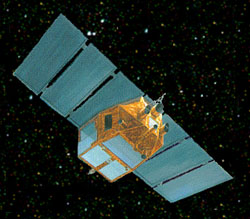
\includegraphics[width=0.30\textwidth]{satellite}
  \end{center}
  \vspace{-20pt}
\end{wrapfigure}
BeppoSAX è un satellite artificiale italo-olandese per l'astronomia a raggi X. Ha apportato importanti contributi nello studio dei lampi gamma o gamma ray burst.

Lanciato dalla base spaziale americana di Cape Canaveral il 30 aprile 1996 con un razzo vettore Atlas-Centaur e realizzato in gran parte da aziende italiane, il satellite chiamato SAX (Satellite per Astronomia a raggi X), una volta in orbita venne ribattezzato BeppoSax, dal soprannome del professor Giuseppe Occhialini (Beppo), un pioniere dell'astrofisica italiana.

Lo scopo fondamentale della missione era studiare le emissioni cosmiche di raggi X, impossibili da studiare da Terra a causa della schermatura dell'atmosfera. In particolare, voleva contribuire allo studio di quei fenomeni cosmici che emettono contemporaneamente radiazioni su un'ampia gamma di livelli energetici, per tentare di comprendere i relativi meccanismi astrofisici.

L'asso nella manica di BeppoSAX era proprio la copertura spettrale (la gamma dei livelli di energia delle emissioni osservabili) particolarmente ampia, che andava da 0,1 a oltre 200 KeV. Si trattava della prima missione capace di studiare sorgenti di raggi X su un intervallo energetico così ampio. In questo modo SAX ha potuto contribuire allo studio di una grande varietà di fenomeni cosmici come sorgenti galattiche compatte, nuclei galattici attivi, ammassi di galassie, resti di supernovae, galassie normali, stelle, gamma ray burst. 

Il satellite è riuscito ad ottenere la prima immagine X di lampo gamma, permettendo di svelarne numerosi segreti. Ad oggi, grazie anche a questo apporto, si ritiene che queste esplosioni di raggi gamma, seconde solo al big bang per valori di energie in gioco, si verifichino ai confini dell'universo conosciuto.

In sei anni di vita operativa ha effettuato oltre 33.000 orbite. Nel 1998 al team scientifico fu conferito il Premio Bruno Rossi, da parte della Società Astronomica Americana. L'importanza della missione consiste soprattutto nell'aver aperto la strada ad un nuovo ed interessante campo di ricerca astronomico.

Il satellite è rientrato nell'atmosfera il 29 aprile 2003, precipitando nell'Oceano Pacifico.

\section*{Osservazioni}
\label{osservazioni}

Nel 1997 dopo aver rivelato un gamma-ray burst (GRB 970228[1]), venne comandato al satellite di puntare la sua apparecchiatura di ricezione di raggi-X nella direzione da cui erano pervenute le emissioni gamma, e lo strumentò rivelò delle emissioni di raggi-X in dissolvenza. Ulteriori osservazioni con telescopi a terra identificarono una debole controparte ottica. Con la posizione della sorgente perfettamente nota, quando l'emissione di raggi gamma si affievolì fino a scomparire, fu possibile raccogliere immagini ottiche più precise fino ad identificare la galassia estremamente lontana che aveva ospitato l'evento - la prima ad essere individuata di molte altre in seguito. Entro poche settimane, la controversia sulle distanze di questi eventi aveva raggiunto una conclusione: i lampi gamma potevano essere finalmente identificati come eventi extra-galattici, che si originavano in galassie molto deboli e ad enormi distanze dalla Terra. Questa scoperta rivoluzionò lo studio dei lampi gamma, stabilendone le distanze, caratterizzando l'ambiente in cui hanno origine e aprendo nuove opportunità osservative e teoriche su di essi.

Utilizzando le osservazioni di Chandra e di BeppoSAX è stato scoperto che la provenienza di molti GRB è associata a zone di formazione stellare.

\section*{Curiosità}
\label{curiosit}

La grande competenza dimostrata in questo campo dalla comunità scientifica e tecnologica italiana (proseguita con la messa in orbita del satellite per astronomia gamma AGILE) ha garantito all'Italia un ruolo di primo piano anche nella missione SWIFT, con cui la NASA spera di risolvere definitivamente il mistero dei gamma-ray burst.

\end{document}